\documentclass[11pt]{scrartcl}
\usepackage{graphicx}
\graphicspath{{./}}
\usepackage[sexy]{evan}
\usepackage[normalem]{ulem}
\usepackage{hyperref}
\usepackage{mathtools}
\hypersetup{
    colorlinks=true,
    linkcolor=blue,
    filecolor=magenta,      
    urlcolor=cyan,
    pdftitle={Overleaf Example},
    pdfpagemode=FullScreen,
    }

\renewcommand{\baselinestretch}{1.5}

\addtolength{\oddsidemargin}{-0.4in}
\addtolength{\evensidemargin}{-0.4in}
\addtolength{\textwidth}{0.8in}
% \addtolength{\topmargin}{-0.2in}
% \addtolength{\textheight}{1in} 

\setlength{\parindent}{0pt}

\usepackage{pgfplots}
\pgfplotsset{compat=1.15}
\usepackage{mathrsfs}
\usetikzlibrary{arrows}

\begin{document}
	\title{Latihan Soal Basic} % Beginner
	\date{\today}
	\author{Azzam L. H.}
	\maketitle
    
    \section{Aljabar}
    \begin{enumerate}
    \item Jika $x=2021^3-2019^3$, maka nilai $\sqrt{\dfrac{x-2}{6}}$ adalah \dots
    \item  dari $\sqrt{5050^2-4950^2}$ adalah \dots

    \item (OSP 2008) Jika $0 < b < a$ dan $a^2+b^2=6ab$, maka nilai $\dfrac{a+b}{a-b}=\dots$
    
    \item Jika $x > 0$ dan $x + \dfrac{1}{x} =  5$, maka nilai $x^3+\dfrac{1}{x^3}$ adalah \dots
    
    \item (OSK 2017) Diketahui $x-y=10$ dan $xy=10$. Nilai $x^4+y^4$ adalah \dots
    
    \item Jika $a+b+c=0$, buktikan bahwa $a^3+b^3+c^3=3abc$.

    \item (AIME 1987)
    Tentukan nilai sederhana dari $\dfrac{(10^4+324)(22^4+324)(34^4+324)(46^4+324)(58^4+324)}{(4^4+324)(16^4+324)(28^4+324)(40^4+324)(52^4+324)}$
    
    \item (OSK 2006) Diketahui $a+(a+1)+(a+2)+\dots+50=1139$. Jika $a$ bilangan real positif, maka $a=\dots$
    
    \item (AIME 1984) Barisan $a_1,a_2,\dots,a_{98}$ memenuhi $a_{n+1}=a_n+1$ untuk $n=1,2,\dots,97$ dan mempunyai jumlah sama dengan $137$. Tentukan nilai dari $a_2+a_4+a_6+\dots+a_{98}$.
    
    \item (AIME 2003) Diketahui $0<a<b<c<d$ adalah bilangan bulat dimana $a,b,c$ membentuk barisan aritmatika sedangkan $b,c,d$ membentuk barisan geometri. Jika $d-a=30$ maka tentukan nilai dari $a+b+c+d$.
    
    \item (OSK 2009) Bilangan bulat positif terkecil $n$ dengan $n> 2009$ sehingga $$\sqrt{\dfrac{1^3+2^3+3^3+\dots+n^3}{n}}$$
    merupakan bilangan bulat adalah \dots
    
    \item Tentukan nilai paling sederhana dari $\sqrt{2\sqrt{2\sqrt{2\sqrt{\dots}}}}$.
    
    \item Tentukan nilai dari $\dfrac{1}{1\cdot2}+\dfrac{1}{2\cdot 3}+\dfrac{1}{3 \cdot 4}+\dots+\dfrac{1}{2020 \cdot 2021}.$
    
    \item  Nilai paling sederhana dari $\left(1-\dfrac{1}{2^2}\right)\cdot\left(1-\dfrac{1}{3^2}\right)\cdot\left(1-\dfrac{1}{4^2}\right)\cdot\dots\cdot\left(1-\dfrac{1}{2021^2}\right)$ adalah \dots
    
    \item Tentukan hasil dari jumlah $\dfrac{1}{\sqrt{1}+\sqrt{2}}+\dfrac{1}{\sqrt{2}+\sqrt{3}}+\dots+\dfrac{1}{\sqrt{99}+\sqrt{100}}.$
    
    \item Nilai $x$ yang memenuhi persamaan
    $$\sqrt{x\sqrt{x\sqrt{x\sqrt{\dots}}}}=\sqrt{4x+\sqrt{4x+\sqrt{4x+\sqrt{\dots}}}}$$
    adalah \dots
    
    \item Hitunglah nilai paling sederhana dari
    $$6-\dfrac{5}{3+\dfrac{4}{3+\dfrac{4}{3+\dfrac{4}{3+\dfrac{4}{\dots}}}}}$$
    
    \item Jika $f:\RR-\{0\} \rightarrow \RR$ adalah fungsi yang memenuhi $f(x)+2f\left(\frac{1}{x}\right)=3x$ untuk setiap bilangan real $x \neq 0$, maka tentukan nilai $f(2021).$
    
    \item (OSP 2004) Misalkan $f$ sebuah fungsi yang memenuhi $f(x)f(y)-f(xy)=x+y,$ untuk setiap bilangan bulat $x$ dan $y$. Berapakah nilai $f(2004)$?
    
    \item (OSK 2011) Misalkan $f$ suatu fungsi yang memenuhi $f(xy) = \dfrac{f(x)}{y}$ untuk semua bilangan real positif $x$ dan $y$. Jika $f(100)=3$ maka $f(10)$ adalah \dots
    
    \item (OSP 2009) Suatu fungsi $f:\ZZ \rightarrow \QQ$ mempunyai sifat $f(x+1)=\dfrac{1+f(x)}{1-f(x)}$ untuk setiap $x \in \ZZ$. Jika $f(2)=2$, maka nilai fungsi $f(2009)$ adalah \dots
    
    \item Jika $P(x)$ dibagi $x^2-x$ dan $x^2+x$ berturut-turut akan bersisa $5x+1$ dan $3x+1$, maka bila $P(x)$ dibagi $x^2-1$ sisanya adalah \dots
    
    \item (OSP 2006) Jika $(x-1)^2$ membagi $ax^4+bx^3+1$, maka $ab=\dots$
    
    \item Diketahui suatu polinomial $P(x)$ memenuhi $P(k)=\dfrac{k}{k+1}$ untuk $k=1,2,3,\dots,2020$. Jika $P(0)=1$, nilai $P(2022)=\dots$
    
    \item (OSK 2010) Polinom $P(x)=x^3-x^2+x-2$ mempunyai tiga pembuat nol yaitu $a,b,$ dan $c$. Nilai dari $a^3+b^3+c^3$ adalah \dots
    
    \item (OSP 2010) Persamaan kuadrat $x^2-px-2p=0$ mempunyai dua akar real $\alpha$ dan $\beta$. Jika $a^3+b^3=16$, maka hasil jumlah semua nilai $p$ yang memenuhi adalah \dots 
    
    \item Diberikan polinomial $P(x)=x^4+ax^3+bx^2+cx+d$ dengan $a,b,c,$ dan $d$ konstanta. Jika $P(1)=10$, $P(2)=20$, dan  $P(3)=30$, maka nilai
    $\dfrac{P(12)+P(-8)}{10}=\dots$
    
    \item Carilah jumlah semua bilangan bulat positif $a$ yang memenuhi $a^{(a-1)^{(a-2)}}=a^{a^2-3a+2}$.
        
        \item Carilah jumlah seluruh solusi real $x$ yang memenuhi $(x^2+5x+5)^{x^2-10x+21}=1.$
        
        \item Jika $5^x=6^y=30^7$, berapakah nilai $\dfrac{xy}{x+y}$?
        
        \item (OSK 2012) Jumlah semua bilangan bulat $x$ sehingga $^2 \log (x^2-4x-1)$ merupakan bilangan bulat adalah \dots
        
        \item (OSK 2014) Misalkan $x,y,z>1$ dan $w>0$. Jika $\log_x w = 4$, $\log_y w = 5$, dan $\log_{xyz} w = 2$, maka nilai $\log_z w$ adalah \dots 
        
        \item (Modifikasi JBMO 2021) Carilah seluruh penyelesaian dari persamaan $2\cdot \lfloor{\frac{1}{2x}}\rfloor - 7 = 9(1 - 8x)$.
        
        \item Banyaknya bilangan asli $n \in \{1,2,3,\dots,1000\}$ sehingga terdapat bilangan real positif $x$ yang memenuhi $x^2+\floor{x}^2=n$ adalah \dots
        
        \item (OSK 2016) Misalkan $x,y,z$ adalah bilangan real positif yang memenuhi $$3 \log_x (3y) = 3 \log_{3x} (27z) = \log_{3x^4} (81yz) \neq 0.$$ Nilai dari $x^5y^4z$ adalah \dots
        
        \item (Nesbitt's Inequality) Untuk bilangan real positif $a,b,c$ tentukan nilai minimum dari $$\dfrac{a}{b+c}+\dfrac{b}{c+a}+\dfrac{c}{a+b}.$$
        
        \item Tentukan nilai minimum dari $8x^4+y^2$ untuk bilangan real positif $x$ dan $y$ yang memenuhi $x^4y=\dfrac{1}{2}$.
        
        \item Nilai minimum dari $$\dfrac{1}{w}+\dfrac{1}{x}+\dfrac{1}{y}+\dfrac{1}{z}$$
        untuk bilangan real positif $w,x,y,z$ yang memenuhi $w+x+y+z=3$ adalah \dots
        
        \item Jika $x^2+y^2+z^2=1$, nilai maksimum dari $x+2y+3z$ adalah \dots
        
        \item Diberikan $a+b+c=1$ dan $a,b,c>0$, carilah nilai minimum dari $a^2+2b^2+c^2$.
        
        \item (OSK 2014) Untuk $0 < x < \pi$, nilai minimum dari $\dfrac{16 \sin^2 x + 9}{\sin x}$ adalah \dots
        
        \item (OSK 2017) Misalkan $a,b,c$ bilangan real positif yang memenuhi $a+b+c=1$. Nilai minimum dari $\dfrac{a+b}{abc}$ adalah \dots
        
        \item (OSK 2017) Pada segitiga $ABC$ titik $K$ dan $L$ berturut-turut adalah titik tengah $AB$ dan $AC$. Jika $CK$ dan $BL$ saling tegak lurus, maka nilai minimum dari $\cot B + \cot C$ adalah \dots
\end{enumerate}


\section{Teori Bilangan}
\begin{enumerate}
    \item (OSN SMP 2003) Buktikan bahwa $(n-1)n(n^3+1)$ selalu habis dibagi 6 untuk semua bilangan asli $n$.
    
    \item Carilah semua bilangan bulat $n$ sehingga $\dfrac{2n+6}{n-1}$ adalah bilangan bulat.
    
    \item (OSK 2002) Bilangan asli $n$ terbesar sehingga $8^n \mid 44^{44}$ adalah \dots
    
    \item Berapa banyak pasangan bilangan bulat positif $(a,b)$ yang memenuhi $\dfrac{1}{a}+\dfrac{1}{b}=\dfrac{1}{6}$.
    
    \item Jika $a$ dan $b$ adalah bilangan bulat sedemikian sehingga $a^2-b^2=2017$, maka nilai dari $a^2+b^2$ adalah \dots
    
    \item (AIME 1986) Tentukan bilangan asli $n$ terbesar sehingga $n+10 \mid n^3+100$.
    
    \item (OSK 2010) Nilai $n$ terkecil sehingga $\underbrace{20102010\dots2010}_\text{$n$ buah 2010}$ habis dibagi 99 adalah \dots
    
    \item Jika dihitung maka didapat $17! = 3a56874280b6000$. Tentukan nilai digit $a$ dan $b$.
    
    \item Tentukan digit satuan dari $7^{7^7}$.
    
    \item Jika $S=1!+2!+3!+\dots+2021!$, tentukan sisa $S$ saat dibagi 6.
    
    \item (OSK 2009) Sisa saat $10^{999999999}$ saat dibagi oleh 7 adalah \dots
    \item (OSK 2011) Bilangan asli terkecil $n>2011$ yang bersisa 1 jika dibagi $2,3,4,5,6,7,8,9,10$ adalah \dots.
    
    \item (OSK 2011) Bilangan asli terkecil lebih dari 2011 yang bersisa 1 jika dibagi 2,3,4,5,6,7,8,9,10 adalah \dots
        
        \item (OSK 2009) Nilai dari $\sum_{k=1}^{2009} FPB(k,7)$ adalah \dots
        
        \item Banyaknya anggota himpunan himpunan 
        $$S = \{gcd(n^3+1,n^2+3n+9 \mid n \in Z\}$$
        adalah \dots
        
        \item (AIME 1998) Ada berapa banyak bilangan bulat positif $k$ sehingga $lcm(6^6,8^8,k)=12^{12}$?
        
        \item Jika $a,b$ adalah bilangan asli dan $c$ adalah bilangan bulat, buktikan bahwa $gcd(a,b)=gcd(a,b+ac).$
        
        \item (OSP 2009) Misalkan $n$ bilangan asli terkecil yang mempunyai tepat 2009 faktor dan $n$ merupakan kelipatan 2009. Faktor prima terkecil dari $n$ adalah \dots
        
        \item Misalkan $n$ bilangan asli dimana $2n$ mempunyai 28 faktor positif dan $3n$ mempunyai 30 faktor positif. Banyaknya faktor positif yang dimilik $6n$ adalah \dots
        
        \item (OSK 2011) Ada berapa faktor positif dari $2^73^55^37^2$ yang merupakan kelipatan 10?
        
        \item (AIME 1995) Tentukan banyaknya faktor positif dari $n^2$ yang kurang dari $n$ tetapi tidak membagi $n$ jika $n^{2^{31}}3^{19}.$
        
        \item (AIME 2000) Tentukan bilangan asli terkecil yang memiliki 12 faktor positif genap dan $6$ faktor positif ganjil.
        
        \item Berapakah sisa pembagian $43^{43^{43}}$ oleh 100?
        
        \item Jika $10^{999999999}$ dibagi oleh 7, maka sisanya adalah \dots
        
        \item Tentukan sisa saat $2^{70}+3^{70}$ saat dibagi 13.
        
        \item Berapa banyak bilangan di himpunan $\{1,2,\dots,200\}$ yang relatif prima dengan 100?
        
        \item Carilah nilai $FPB(19!+19,20!+19).$
        
        \item (OSK 2012) Banyaknya bilangan bulat $n$ yang memenuhi $$(n-1)(n-3)(n-5)\dots(n-2013)=n(n+2)(n+4)\dots (n+2012)$$ adalah \dots
            
            \item (OSK 2013) Diketahui $x_1,x_2$ adalah dua bilangan bulat berbeda yang merupakan akar-akar dari persamaan kuadrat $x^2+px+q+1=0$. Jika $p$ dan $p^2+q^2$ adalah bilangan-bilangan prima, maka nilai terbesar yang mungkin dari $x_1^{2013}+x_2^{2013}$ adalah \dots
            
            \item (OSK 2014) Diberikan tiga bilangan bulat positif berurutan. Jika bilangan pertama tetap, bilangan kedua ditambah 10 dan bilangan ketiga ditambah bilangan prima, maka ketiga bilangan ini membentuk deret ukur. Bilangan ketiga dari bilangan bulat berurutan adalah \dots
            
            \item (OSK 2014) Semua pasangan bilangan prima $(p,q)$ yang memenuhi persamaan
            $$(7p-q)^2=2(p-1)q^2$$
            adalah \dots
            
            \item (OSK 2014) Semua bilangan bulat $n$ sehingga $n^4-51n^2+225$ merupakan bilangan prima adalah \dots
\end{enumerate}

\section{Kombinatorika}
\begin{enumerate}
    \item Misalkan terdapat 3 buah celana dan 4 buah baju. Permasalahannya adalah ada berapa banyak cara 
seseorang memilih celana dan baju yang akan dipakai ?

    \item Berapa banyak cara menyusun huruf-huruf R, A, J, I, N jika 
\begin{enumerate}
    \item huruf pertama dimulai dari huruf hidup (vokal) 
    \item huruf pertama dimulai dari huruf mati (konsonan) 
\end{enumerate}

    \item Sembilan orang siswa akan duduk pada 5 kursi sejajar. Ada berapa cara susunan mereka ? 
    
    \item Denny akan membentuk bilangan genap 3 angka yang angka-angkanya diambil dari 2, 3, 4, 5, 6, 7, 8. 
Berapa banyak bilangan yang dapat dibentuk jika : 
    \begin{enumerate}
        \item angka-angkanya boleh berulang 
\item angka-angkanya tidak boleh berulang
    \end{enumerate}
    
    \item (OSK 2003) Ada berapa banyak bilangan 4-angka (digit) yang semua angkanya genap dan bukan 
merupakan kelipatan 2003 ?
    \item  Carilah banyaknya menempatkan 3 benteng (rooks) pada papan catur $5 \times 5$ sehingga
tidak ada dua catur yang dalam posisi dapat saling menyerang.

    \item Sekumpulan orang duduk mengelilingi sebuah meja bundar. Diketahui ada 7 wanita
dimana di sebelah kanan setiap wanita tersebut adalah wanita dan ada 12 wanita yang di
sebelah kanan setiap wanita tersebut adalah pria. Diketahui pula bahwa 3 dari 4 pria di
sebelah kanannya adalah wanita. Berapa orang yang duduk mengelilingi meja tersebut?

    \item Carilah banyaknya kuadrupel terurut bilangan ganjil positif $(x_1, x_2, x_3, x_4)$ yang memenuhi
$x_1 + x_2 + x_3 + x_4 = 98$.

    \item Perhatikan gambar berikut.\\
    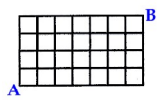
\includegraphics[scale=1.2]{kombin.PNG}
    Jika seseorang akan berjalan dari titik A ke titik B. Ada berapa banyak cara jalan terpendek 
yang dapat dipilihnya ?
    
    \item (OSP 2003) Empat pasang suami istri menonton pagelaran orkestra. Tempat duduk mereka harus 
dipisah antara kelompok suami dan kelompok istri. Untuk masing-masing kelompok disediakan 4
buah tempat duduk bersebelahan dalam satu barisan. Ada berapa banyak cara memberikan 
tempat duduk kepada mereka ?

    \item (OSK 2010) Banyaknya himpunan $X$ yang memenuhi 
$$\{1,2,\dots,1000\} \subseteq X \subseteq \{1,2,\dots,2010\}.$$

    \item (OSP 2010) Bilangan enam digit $abcdef$ dengan $a > b > c \ge d > e > f$ ada sebanyak \dots
    
    \item (OSK 2017)
	Sebuah hotel mempunyai kamar bernomor 000 sampai dengan 999. Hotel tersebut menerapkan
aturan aneh sebagai berikut: jika suatu kamar berisi tamu, dan sembarang dua digit nomor kamar
tersebut dipertukarkan tempatnya, maka diperoleh nomor kamar yang sama atau nomor kamar
yang tidak berisi tamu. Maksimal banyaknya kamar yang berisi tamu adalah \dots

    \item Carilah koefisien $x^4$ dari penjabaran $(x+1)^9$
    
    \item (OSK 2013) Koefisien $x^{2013}$ pada ekspansi
    $$(1+x)^{4026}+x(1+x)^{4025}+x^2(1+x)^{4024}+\dots x^{2013}(1+x)^{2013}$$
    adalah \dots
    
    \item Jika $S=(\sqrt{71}+1)^{71}-(\sqrt{71}-1)^{71}$ adalah bilangan bulat, carilah digit terakhir dari $S$
    \item Berapa banyak orang minimum yang harus hadir di suatu pesta sehingga dipastikan terdapat 3 orang yang lahir di bulan yang sama di pesta itu?
    
    \item Misalkan Naruko memilih $k$ buah bilangan dari himpunan $\{1,2,3,\dots,2016\}$ secara acak. Berapakah nilai $k$ terkecil sehingga Naruko pasti bisa mendapatkan setidaknya sepasang bilangan (dari $k$ bilangan itu) yang jika dijumlahkan hasilnya 2017?
    
    \item Suatu malam di rumah WonYoung terjadi pemadaman listrik. Karena WonYoung sangat malas, ia hanya ingin tidur dengan membawa banyak kaus kaki (hobi yang aneh :/). Ia mengambil kaus kaki dari lemari di ruangan yang sangat gelap. Lemari itu berisi 100 buah kaus kaki merah, 80 kaus kaki hijau, 60 kaus kaki biru, dan 40 kaus kaki hitam. WonYoung mengambil banyak kaus kaki tapi tidak bisa tahu warnanya. Berapa banyak kaus kaki paling sedikit yang perlu diambil sehingga dijamin terdapat setidaknya 10 pasang kaus kaki (dengan setiap pasang kaus kaki harus berwarna sama) ?
    
    \item (OSK 2011) Di lemari hanya ada 2 macam kaos kaki yaitu kaos kaki berwarna hitam dan putih. 
Ali, Budi dan Candra berangkat di malam hari saat mati lampu dan mereka mengambil kaos kaki 
secara acak di dalam lemari dalam kegelapan. Berapa kaos kaki minimal harus mereka ambil untuk 
memastikan bahwa akan ada tiga pasang kaos kaki yang bisa mereka pakai ? (Sepasang kaos kaki harus 
memiliki warna yang sama).
    
    \item Tandai satu buah kartu dengan angka 1, dua buah kartu dengan angka 2, tiga buah kartu dengan 
angka satu hingga lima puluh buah kartu dengan angka 50. Semua kartu tersebut dimasukkan ke dalam kotak. Berapa buah kartu minimal yang harus diambil agar dapat dipastikan terdapat sekurang-kurangnya 10 buah kartu dengan tanda angka yang sama 

    \item (OSK 2016)
	Anak laki-laki dan anak perempuan yang berjumlah 48 orang duduk melingkar secara acak.
Banyaknya minimum anak perempuan sehingga pasti ada enam anak perempuan yang duduk
berdekatan tanpa diselingi anak laki-laki adalah \dots

    \item (OSK 2012) Suatu set soal terdiri dari 10 soal pilihan B atau S dan 15 soal pilihan ganda dengan 4 pilihan. Seorang siswa menjawab semua soal dengan menebak jawaban secara acak. Tentukan probabilitas ia menjawab dengan benar hanya 2 soal.
            
            \item (OSK 2012) Misalkan terdapat 5 kartu dimana setiap kartu diberi nomor yang berbeda yaitu 2, 3, 4, 5, 6. Kartu-kartu tersebut kemudian dijajarkan dari kiri ke kanan secara acak sehingga berbentuk barisan. Berapa probabilitas bahwa banyaknya kartu yang dijajarkan dari kiri ke kanan dan ditempatkan pada tempat ke- $i$ akan lebih besar atau sama dengan $i$ untuk setiap $i$ dengan $1 \le i \le 5$ ?
            
            \item (OSK 2013) Suatu dadu ditos enam kali. Banyak cara memperoleh jumlah mata yang muncul 28 dengan tepat satu dadu muncul angka 6 adalah \dots
            
            \item (OSK 2013) Sepuluh kartu ditulis dengan angka satu sampai sepuluh (setiap kartu hanya terdapat satu angka dan tidak ada dua kartu yang memiliki angka yang sama). Kartu - kartu tersebut dimasukkan kedalam kotak dan diambil satu secara acak. Kemudian sebuah dadu dilempar. Probabilitas dari hasil kali angka pada kartu dan angka pada dadu menghasilkan bilangan kuadrat adalah \dots
            
            \item (OSK 2018) Diberikan satu koin yang tidak seimbang. Bila koin tersebut ditos satu kali, peluang muncul angka adalah $\frac{1}{4}$. Jika ditos $n$ kali, peluang muncul tepat dua angka sama dengan peluang muncul tepat tiga angka. Nilai $n$ adalah \dots
            
            \item (OSK 2017) Pada suatu kotak ada sekumpulan bola berwarna merah dan hitam yang secara keseluruhannya kurang dari 1000 bola. Misalkan diambil dua bola. Peluang terambilnya dua bola merah adalah $p$ dan peluang terambilnya dua bola hitam adalah $q$ dengan $p-q =\frac{23}{37}$. Selisih terbesar yang mungkin dari banyaknya bola merah dan hitam adalah \dots
            
            \item (OSK 2017) Terdapat enam anak, $A, B, C, D, E$ dan $F$, akan saling bertukar kado. Tidak ada yang menerima kadonya sendiri, dan kado dari $A$ diberikan kepada $B$. Banyaknya cara membagikan kado dengan cara demikian adalah \dots
\end{enumerate}

\section{Geometri}
\begin{enumerate}
    \item Pada segiempat $WXYZ$ dengan diagonal yang saling tegak lurus diketahui bahwa $\angle WZX = 30^\circ, \angle XWY = 40^\circ,$ and $\angle WYZ = 50^\circ$. Hitunglah besar $\angle X$ dan $\angle Z$.
    
    \item
		Garis berat $AD$ pada segitiga $ABC$ memotong garis berat $CF$ di titik $P$, serta perpanjangan $BP$ memotong $AC$ di $E$. Jika diketahui segitiga $ABC$ lancip dan $AB=6$, maka panjang $DE$ adalah \dots
		
	\item (OSK 2013) Diberikan segitiga lancip $ABC$ dengan $O$ sebagai pusat lingkaran luarnya. Misalkan $M$ dan $N$
berturut - turut pertengahan $OA$ dan $BC$. Jika $\angle ABC = 4\angle OMN$ dan $\angle ACB = 6\angle OMN$,
maka besarnya $\angle OMN$ sama dengan \dots

    \item (\textbf{Soal Legend: OSK 2011,2012,2013,2018}) Diberikan segitiga $ABC$ dan lingkaran $\Gamma$ yang berdiameter $AB$ . Lingkaran $\Gamma$ memotong sisi $AC$ dan $BC$
berturut-turut di titik $D$ dan $E$. Jika $AD = \frac13 AC, BE =\frac14 BC$ dan $AB = 30$, maka luas segitiga $ABC$ adalah \dots
		
	\item
		Diberikan segitiga $ABC$ dengan $D$ titik tengah $AC$, $E$ titik tengah $BD$, dan $H$ merupakan pencerminan $A$ terhadap $E$. Jika $F$ merupakan perpotongan antara $AH$ dengan $BC$, maka nilai $\dfrac{AF}{FH}$ sama dengan \dots
		
	\item 	
		 Pada gambar di bawah, diketahui titik A $\ne$ B pada lingkaran berdiameter $MN$ dan berpusat di $C$. $P$ adalah titik pada segmen $CN$ dimana $\angle CAP = \angle CBP = 10 ^\circ$. Jika $\angle ACM = 40^\circ$, maka $\angle BCN = \dots^\circ$
		 
		 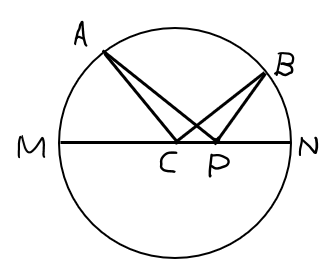
\includegraphics[scale=0.7]{pemanasan post test geom}
		 
	\item
		Diberikan sebuah segitiga dengan panjang sisi $BC = 20$, $CA = 24$, dan $AB=12$. Titik $D$ pada segmen $BC$ dengan $BD = 5$. Lingkaran luar dari segitiga $ABD$ memotong $CA$ di $E$. Hitunglah nilai $2 \times DE$.
		
	\item Jika $A+B=45^\circ$ dan $\cos A\sin B=\frac{\sqrt{2}}{6}$, maka $\cos(B-A)=\dots$
	
	\item Nilai dari $\cos \dfrac{\pi}{7}\cdot \cos \dfrac{2\pi}{7} \cdot \cos \dfrac{4\pi}{7}$ adalah \dots
	
	\item Pada segitiga $ABC$, buktikan bahwa $\tan A + \tan B + \tan C = \tan A \tan B \tan C$.
	
	\item Tentukan nilai eksak dari $\tan 1^\circ \cdot \tan 2^\circ \cdot \tan 3^\circ \cdot \ldots \cdot \tan 89^\circ$.
	
	\item (OSK 2005) Nilai dari $\sin^8 75^\circ - \cos^8 75^\circ$ adalah \dots
	
	\item (OSK 2006) Pada segitiga $ABC$, titik $F$ membagi sisi $AC$ dalam perbandingan $1 : 2$. 
Misalkan $G$ titik tengah $BF$ dan $E$ titik perpotongan antara sisi $BC$ dengan $AG$. Maka titik $E$ membagi sisi $BC$
dalam perbandingan \dots

\item (OSK 2009) Diberikan persegi $ABCD$ dengan panjang sisi 10. Misalkan $E$ pada $AB$ dan $F$
pada $BC$ dengan $AE = FB = 5$. Misalkan $P$ adalah titik potong $DE$ dan $AF$. Luas $DCFP$ adalah \dots

\item (OSN 2011 SMP/MTs) Bangun datar $ABCD$ adalah
trapesium dengan $AB$ sejajar $CD$ dan $AB < CD$. Titik $E$ dan $F$ terletak
pada $CD$ sehingga $AD$ sejajar $BE$ dan $AF$ sejajar $BC$. Titik $H$ 
adalah perpotongan $AF$ dengan $BE$ dan titik $G$ adalah 
perpotongan $AC$ dengan $BE$. Jika panjang $AB$ adalah 4 cm
dan panjang $CD$ adalah 10 cm hitunglah perbandingan luas 
segitiga $AGH$ dengan luas trapesium $ABCD$. 

\item Pada segitiga $ABC$, titik $D$ dan $E$ berturut-turut berada di segmen $AB$ dan $AC$. Misalkan $CD$ dan $BE$ berpotongan di titik $F$. Jika $[DBF]=3$, $[BFC]=6$, dan $[CFE]=4$, berapakah luas $ADFE$?

\item (OSK 2016) Pada segitiga ABC, titik $X, Y$ dan $Z$ berturut-turut terletak pada sinar $BA, CB$ dan $AC$
	sehingga $BX = 2BA, CY = 2CB$ dan $AZ = 2AC$. Jika luas segitiga $ABC$ adalah 1, maka luas
	segitiga $XYZ$ adalah \dots
	
\item (OSK 2016) Segitiga $ABC$ merupakan segitiga sama kaki dengan panjang $AB = AC = 10 $.
	Titik $D$ terletak pada garis $AB$ sejauh $7 $ dari $A$ dan $E$ titik pada garis $AC$ yang
	terletak sejauh $4 $ dari $A$. Dari $A$ ditarik garis tinggi dan memotong $BC$ di $F$.
	Jika bilangan rasional $\frac{a}{b}$ menyatakan perbandingan luas segi empat $ADFE$ terhadap
	luas segitiga $ABC$ dalam bentuk yang paling sederhana, maka nilai $a + b$ adalah \dots
	
	\item (OSK 2014) Diberikan segitiga $ABC$ dengan $AB = 360, BC = 240,$ dan $AC = 180$. Garis
	bagi dalam dan garis bagi luar dari $\angle CAB$ memotong $BC$ dan perpanjangan $BC$
	berturut-turut di $P$ dan $Q$. Jari-jari lingkaran yang melalui titik-titik $A, P,$ dan $Q$
	adalah \dots
	
	\item (OSK 2012) Diketahui $\triangle ABC$ sama kaki dengan panjang $AB = AC = 3$, $BC = 2$, titik $D$ pada sisi $AC$ dengan panjang $AD = 1$. Tentukan luas $\triangle ABD$.
            
            \item (OSK 2016) Diberikan empat titik pada satu lingkaran $\Gamma$ dalam urutan $A,B,C,D$. Sinar garis $AB$ dan $DC$ berpotongan di $E$, dan sinar garis $AD$ dan $BC$ berpotongan di $F$. Misalkan $EP$ dan $FQ$ menyinggung lingkaran $\Gamma$ berturut-turut di $P$ dan $Q$. Misalkan pula bahwa $EP=60$ dan $FQ=63$, maka panjang $EF$ adalah \dots
            
            \item (OSK 2013) Misalkan $P$ adalah titik interior dalam daerah segitiga $ABC$ sehingga besar $\angle PAB = 10^\circ, \angle PBA = 20^\circ, \angle PCA = 30^\circ, \angle PAC=40^\circ$. Besar $\angle ABC = \dots$
            
            \item (OSK 2012) Diberikan segitiga $ABC$ dengan keliling 3, dan jumlah kuadrat sisi-sisinya sama dengan 5. Jika jari-jari lingkaran luarnya sama dengan 1, maka jumlah ketiga garis tinggi dari segitiga $ABC$ tersebut adalah \dots
            
            \item (OSK 2014) Diberikan segitiga $ABC$ yang sisi-sisinya tidak sama panjang sehingga panjang garis berat $AN$ dan $BP$ berturut-turut 3 dan 6. Jika luas segitiga $ABC$ adalah $3\sqrt{15}$, maka panjang garis berat ketiga $CM$ adalah \dots
            
            \item (OSK 2016) Pada segitiga $ABC$, titik $M$ terletak pada $BC$ sehingga $AB=7, AM=3, BM=5$, dan $MC=6$. Panjang $AC$ adalah \dots
            
            \item Diberikan sebuah segiempat siklis $ABCD$ dengan $ABC$ adalah segitiga sama sisi. Jika $AD=2$ dan $CD=3$, panjang $BD=\dots$
            
            \item (OSK 2017) Pada sebuah lingkaran dengan pusat $O$, talibusur $AB$ berjarak 5 dari titik $O$ dan talibusur $AC$ berjarak $5\sqrt{2}$ dari titik $O$. Jika panjang jari-jari lingkaran 10, maka $BC^2=\dots$
\end{enumerate}
    
\end{document}